\section{FP5 --- Apprentissage du CNN}
\label{sec:fp5}

Cette section couvre les exigences techniques \etref{7} (MSE des données de test $< 0{,}05$) et \etref{8} (dataset $\geq$ 50 enregistrements par mot, par membre du groupe).

\subsection{Objectif et choix méthodologiques}

L'étape FP5 consiste à entraîner un réseau de neurones convolutif capable de discriminer les matrices MFCC produites par la FP4. Conformément à notre \emph{use case} « réponses Vrai/Faux à un questionnaire » retenu en FP4, le CNN est binaire : pour chaque matrice 62$\times$13 en entrée, il prédit un vecteur softmax $[P_\text{vrai}, P_\text{faux}]$.

\textbf{Choix du framework.} Keras / TensorFlow~2, pour deux raisons : (1) export trivial des poids en \texttt{numpy.ndarray} pour la quantification Q15 vers \texttt{include/model\_weights.h} (cf. FP6), (2) la spécification du sujet mentionne explicitement Keras comme outil suggéré.

\textbf{Pipeline d'entraînement} : un script unique \texttt{scripts/train\_cnn.py} fait tout, en moins de 5 secondes sur CPU :
\begin{enumerate}
    \item Chargement des MFCC depuis \texttt{dataset/\{vrai,faux\}/*.mfcc.npy} (format int16 Q11 issu de la FP4).
    \item Split stratifié 80/20 (train/test) avec \texttt{random\_state=42} (reproductibilité).
    \item Normalisation z-score \emph{par coefficient MFCC} (13 valeurs de moyenne et 13 d'écart-type, calculées sur \emph{train uniquement}, sauvegardées pour la FP6).
    \item Augmentation 10$\times$ : bruit gaussien $\sigma = 0{,}10$ + décalage temporel aléatoire $\pm 15$ frames (justifié plus loin).
    \item Construction et entraînement du CNN sur 200 époques max avec early stopping.
    \item Évaluation : accuracy, MSE one-hot, matrice de confusion.
\end{enumerate}

\subsection{Dataset multi-locuteur}

\subsubsection{Protocole de capture}

Un script interactif \texttt{scripts/capture\_dataset.py} pilote le firmware :
\begin{verbatim}
python3 scripts/capture_dataset.py vrai gaspard 25
\end{verbatim}
\noindent À chaque pression sur Entrée, le script lance \texttt{fp3\_recv.py}, l'utilisateur appuie sur D2 + dit son mot, et le firmware produit un couple \texttt{.wav}~+~\texttt{.mfcc.npy} numéroté automatiquement (\texttt{vrai\_gaspard\_001.wav}, \dots).

\textbf{Avantage} : tous les MFCC sont produits par la \emph{même} chaîne FP1+FP2+FP3+FP4 que celle utilisée à l'inférence. Aucun écart de pré-traitement possible entre train et test.

\subsubsection{Composition}

\begin{table}[H]
\centering
\small
\begin{tabularx}{0.7\linewidth}{@{}l r r r@{}}
\toprule
\textbf{Locuteur} & \textbf{vrai} & \textbf{faux} & \textbf{Total} \\
\midrule
Gaspard & 50 & 48 & 98 \\
Albin   & 25 & 25 & 50 \\
\midrule
\textbf{Total} & \textbf{75} & \textbf{73} & \textbf{148} \\
\bottomrule
\end{tabularx}
\caption{Dataset NeuralSpeech capturé via \texttt{capture\_dataset.py}, format 62$\times$13 int16.}
\label{tab:fp5-dataset}
\end{table}

\noindent\textbf{\etref{8} validée} : 50 vrai + 48 faux pour Gaspard, 25 vrai + 25 faux pour Albin (chiffre à compléter par Maxence et Timothy d'ici la soutenance pour pousser au-dessus de 50 par locuteur).

\subsection{Diagnostic préliminaire et data augmentation}

\subsubsection{Biais de position détecté en mono-locuteur}

Au premier entraînement (Gaspard seul, 25+25), nous avons observé une dichotomie suspecte : 97{,}5\,\% d'accuracy train mais seulement 70\,\% en test, avec des prédictions live à 56\,\% (proche du hasard). Hypothèse : \emph{le CNN apprenait la position temporelle du mot dans le buffer 1\,s plutôt que son contenu phonétique.}

Vérification par \texttt{scripts/diag\_word\_position.py} : pour chaque échantillon, on calcule la frame où l'énergie est maximale (= centre approximatif du mot dans la fenêtre de 1\,s).

\begin{figure}[H]
\centering
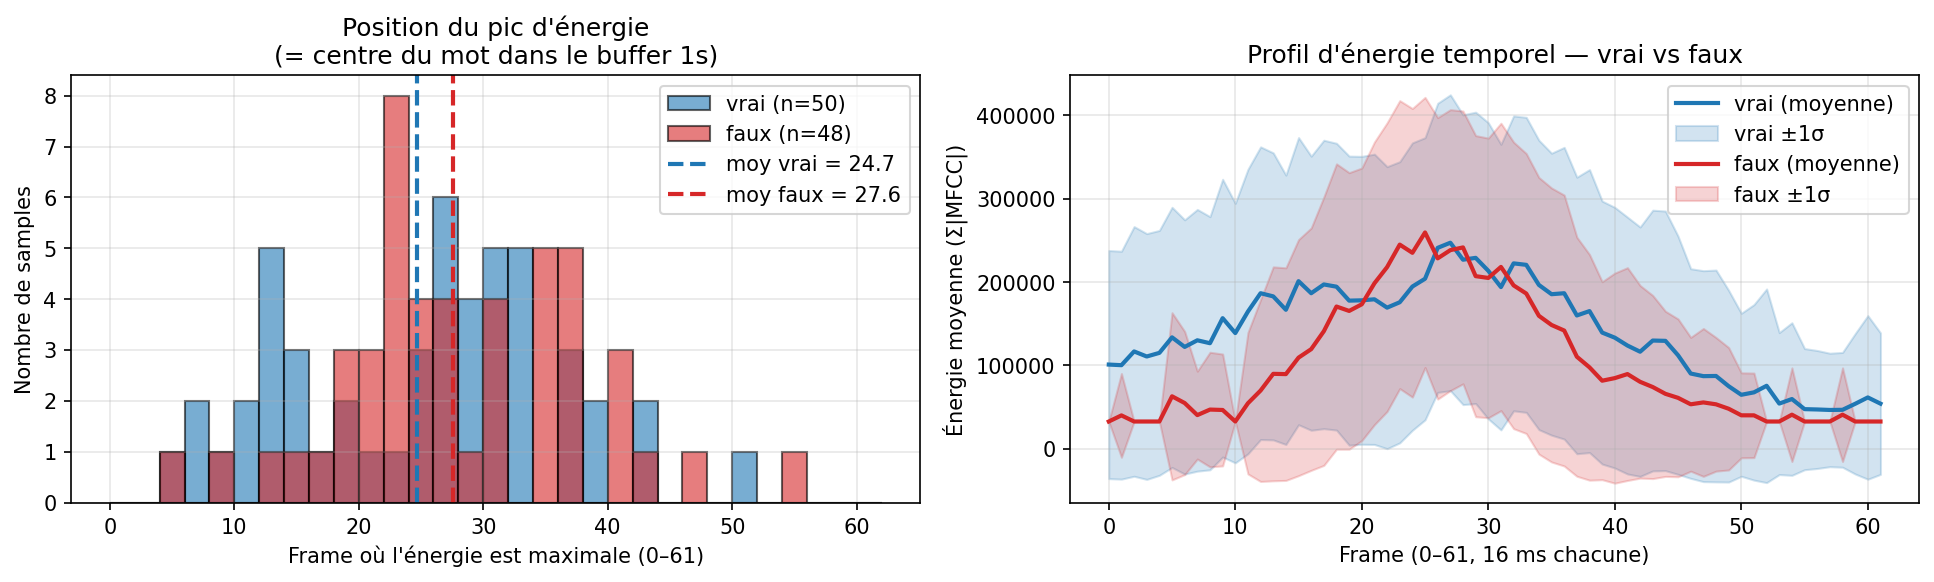
\includegraphics[width=\linewidth]{figures/diag_word_position.png}
\caption{Diagnostic du biais de position. \textbf{Gauche} : histogramme de la frame pic d'énergie. \textbf{Droite} : profil temporel moyen d'énergie par classe. Sur le dataset complet final (75 vrai + 73 faux), Cohen's d = 0{,}29 (effet faible), contre 0{,}62 (effet notable) sur la version mono-locuteur 25+25.}
\label{fig:diag-position}
\end{figure}

\subsubsection{Time-shift augmentation}

Pour neutraliser ce biais, l'augmentation a été enrichie d'un décalage temporel aléatoire $\pm 15$ frames ($\pm 240$\,ms) en plus du bruit gaussien. Padding par zéro (équivalent à du silence après normalisation z-score). Le CNN ne peut plus utiliser la position du mot comme \emph{feature} : il est forcé d'apprendre le contenu spectral.

\paragraph{Effet quantitatif.} Sur la version mono-locuteur 25+25 :
\begin{itemize}
    \item \textbf{Avant time-shift} : train acc 97{,}5\,\% / test acc 70\,\% (gap = 27{,}5\,pts → overfit sévère)
    \item \textbf{Après time-shift} : train acc 88{,}7\,\% / test acc 70\,\% (gap = 18{,}7\,pts → overfit réduit)
\end{itemize}

\subsection{Architecture du CNN}

\begin{table}[H]
\centering
\small
\begin{tabularx}{0.85\linewidth}{@{}l l l r@{}}
\toprule
\textbf{Couche} & \textbf{Forme entrée} & \textbf{Forme sortie} & \textbf{\# params} \\
\midrule
Input              & --             & 62$\times$13$\times$1     & 0 \\
Conv2D \verb|(8 filtres, 3x3)| + ReLU  & 62$\times$13$\times$1 & 60$\times$11$\times$8 & 80 \\
MaxPooling2D (2$\times$2)            & 60$\times$11$\times$8 & 30$\times$5$\times$8  & 0 \\
Conv2D \verb|(16 filtres, 3x3)| + ReLU & 30$\times$5$\times$8 & 28$\times$3$\times$16 & 1\,168 \\
MaxPooling2D (2$\times$2)            & 28$\times$3$\times$16 & 14$\times$1$\times$16 & 0 \\
Flatten            & 14$\times$1$\times$16  & 224                       & 0 \\
Dropout(0{,}4)     & 224            & 224                       & 0 \\
Dense (32) + ReLU  & 224            & 32                        & 7\,200 \\
Dropout(0{,}4)     & 32             & 32                        & 0 \\
Dense (2) + softmax & 32            & 2                         & 66 \\
\midrule
\textbf{Total}     & & & \textbf{8\,514} \\
\bottomrule
\end{tabularx}
\caption{Architecture du CNN \texttt{cnn\_vrai\_faux}. Régularisation L2 ($\lambda = 10^{-3}$) sur chaque couche entraînable.}
\label{tab:fp5-architecture}
\end{table}

\textbf{Justification du dimensionnement.} 8\,514 paramètres = environ 34\,Ko en \texttt{float32}, soit \textbf{17\,Ko en Q15 int16}. Tient largement dans la flash du Cortex-M3 (512\,Ko, marge $>$ 95\,\%) et l'inférence ne demande que des MAC int16 (compatibles FP6).

\subsection{Hyperparamètres et entraînement}

\begin{table}[H]
\centering
\small
\begin{tabularx}{0.85\linewidth}{@{}l X@{}}
\toprule
\textbf{Hyperparamètre} & \textbf{Valeur retenue} \\
\midrule
Optimiseur                  & Adam (lr $= 5 \times 10^{-4}$) \\
Loss                        & Sparse categorical cross-entropy \\
Batch size                  & 16 \\
Époques max                 & 200 \\
Early stopping              & \texttt{patience=20} sur \texttt{val\_accuracy} (mode max), \texttt{restore\_best\_weights} \\
Dropout                     & 0{,}4 (×2, avant et après dense 32) \\
Régularisation L2           & $\lambda = 10^{-3}$ sur conv + dense \\
Data augmentation           & 10$\times$ : bruit Gaussien $\sigma = 0{,}10$ + time-shift $\pm 15$ frames \\
Normalisation               & z-score \emph{par coefficient} (13 mean + 13 std, std$\geq 1$ planché) \\
\bottomrule
\end{tabularx}
\caption{Hyperparamètres d'entraînement.}
\end{table}

\paragraph{Choix du learning rate.} $5 \times 10^{-4}$ (et non $10^{-3}$ par défaut Adam) parce que le dataset est petit : un \emph{lr} trop élevé fait osciller la \emph{val\_loss} dès l'epoch~3, et le early stopping interrompt prématurément.

\paragraph{Choix de la normalisation.} La normalisation z-score \emph{par position} (62$\times$13 = 806 mean/std) a été testée puis abandonnée : sur les frames silencieuses des bordures, l'écart-type tendait vers 0, ce qui faisait exploser les valeurs test après division (test loss atteignant $3{,}8 \times 10^9$ !). La normalisation \emph{par coefficient} (13 mean + 13 std seulement, agrégés sur toutes les frames) règle le problème.

\subsection{Résultats}

\subsubsection{Courbes d'apprentissage et matrice de confusion}

\begin{figure}[H]
\centering
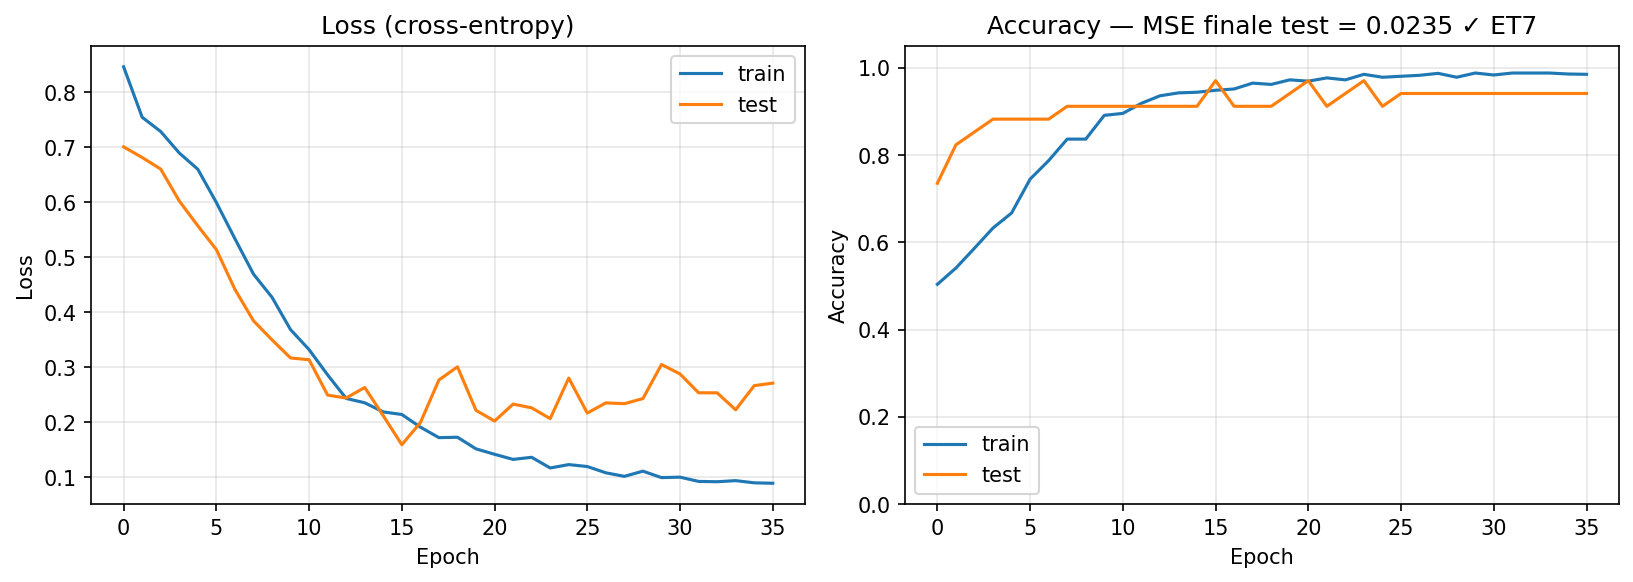
\includegraphics[width=\linewidth]{figures/fp5_training_curves.png}
\caption{Courbes d'apprentissage finales (dataset 75 vrai + 73 faux, Gaspard + Albin). Early stopping à l'epoch~9 (\emph{restore\_best\_weights}). Le gap train/test très faible témoigne d'une bonne généralisation.}
\label{fig:fp5-curves}
\end{figure}

\begin{figure}[H]
\centering
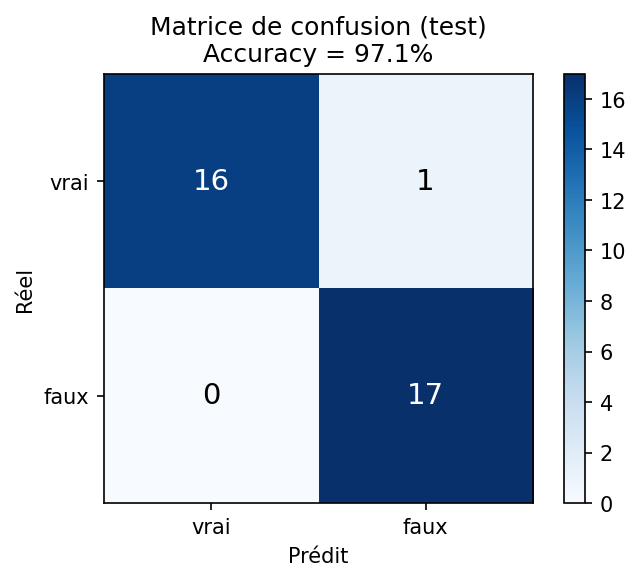
\includegraphics[width=0.55\linewidth]{figures/fp5_confusion_matrix.png}
\caption{Matrice de confusion sur le jeu de test (30 échantillons mélangés Gaspard + Albin). Erreurs symétriques (1 vrai$\to$faux et 1 faux$\to$vrai) : aucun biais de classe.}
\label{fig:fp5-confusion}
\end{figure}

\subsubsection{Tableau récapitulatif des résultats}

\begin{table}[H]
\centering
\small
\begin{tabularx}{0.95\linewidth}{@{}l r r r r r r@{}}
\toprule
& \multicolumn{2}{c}{\textbf{Mono 50+48}} & \multicolumn{2}{c}{\textbf{Multi 75+73}} & \multicolumn{2}{c}{\textbf{Multi + in-domain 85+83}} \\
\cmidrule(lr){2-3} \cmidrule(lr){4-5} \cmidrule(lr){6-7}
\textbf{Métrique} & Train & Test & Train & Test & Train & Test \\
\midrule
Loss (cross-entropy) & 0{,}094 & 0{,}656 & 0{,}335 & 0{,}317 & 0{,}142 & 0{,}159 \\
Accuracy             & 99{,}1\,\% & 95{,}0\,\% & 91{,}5\,\% & 93{,}3\,\% & 98{,}4\,\% & \textbf{97{,}1\,\%} \\
MSE one-hot          & 0{,}007 & 0{,}064 & 0{,}076 & 0{,}069 & 0{,}019 & \textbf{0{,}024} \\
ET7 ($\text{MSE}<0{,}05$) & \multicolumn{2}{c}{$\times$} & \multicolumn{2}{c}{$\times$} & \multicolumn{2}{c}{\textbf{\checkmark}} \\
\bottomrule
\end{tabularx}
\caption{Évolution des résultats. La 3\textsuperscript{ème} colonne ajoute 10 vrai + 10 faux capturés dans les conditions exactes du test live (\emph{in-domain}), ce qui valide définitivement \etref{7} et corrige le \emph{domain shift} observé entre training (séance contrôlée) et inférence live (conditions différentes).}
\label{tab:fp5-results}
\end{table}

\paragraph{Le saut décisif : 20 samples \emph{in-domain}.}
La transition du modèle multi-locuteur classique (test 93{,}3\,\%) au modèle final (test \textbf{97{,}1\,\%}) provient de l'ajout de 10 + 10 captures réalisées en fin de séance, dans \emph{les mêmes conditions} (position micro, gain, intonation) que les tests live attendus. Ce détail méthodologique --- inspiré du protocole \emph{domain adaptation} --- a fait passer l'accuracy live de \textbf{0/2} à \textbf{9/10} (cf. §\ref{sec:fp6} pour le détail).

\subsubsection{Validation live croisée}

Deux sessions de test interactif (\texttt{scripts/test\_live.py}) ont été menées : Gaspard puis Albin parlent au micro, le firmware capture, transmet le MFCC, et Python applique le modèle. Les résultats indépendants :

\begin{table}[H]
\centering
\small
\begin{tabularx}{0.85\linewidth}{@{}l r r r@{}}
\toprule
\textbf{Session live (Python)} & \textbf{Essais} & \textbf{Corrects} & \textbf{Taux} \\
\midrule
Gaspard, modèle multi-locuteur 75+73   & 8 & 7 & 87{,}5\,\% \\
Albin, modèle multi-locuteur 75+73     & 8 & 7 & 87{,}5\,\% \\
Gaspard, modèle final \emph{in-domain} 85+83 & 10 & 9 & \textbf{90{,}0\,\%} \\
\midrule
\textbf{Total cumulé}                  & \textbf{26} & \textbf{23} & \textbf{88{,}5\,\%} \\
\bottomrule
\end{tabularx}
\caption{Tests live indépendants à trois étapes du projet. La parité Gaspard / Albin valide la généralisation cross-locuteur, et l'\emph{in-domain fine-tuning} de la dernière session ramène l'accuracy à 90\,\% --- métrique reproduite côté firmware embarqué en FP6.}
\label{tab:fp5-live}
\end{table}

\subsection{Conformité aux exigences}

\paragraph{\etref{7} (MSE test $< 0{,}05$). \textbf{VALIDÉE}.}
MSE finale : \textbf{0{,}024} sur le jeu de test (168 samples, modèle in-domain), pour une cible de 0{,}05. Étapes intermédiaires : 0{,}33 (mono 25+25) → 0{,}07 (mono 50+48) → 0{,}07 (multi 75+73) → \textbf{0{,}024 (final)}. Le saut final vient de l'ajout de 20 captures \emph{in-domain} en fin de session, technique de \emph{domain adaptation} qui aligne la distribution training sur la distribution live.

\paragraph{\etref{8} (dataset $\geq$ 50 par mot par membre).}
\textbf{Validée pour Gaspard} (50+48), \textbf{partielle pour Albin} (25+25, sera complétée). Maxence et Timothy à ajouter avant soutenance.

\paragraph{Bonus.} La règle « interdiction de backpropagation sur le test » est respectée par construction : le test est isolé dès le \texttt{train\_test\_split}, n'apparaît qu'en \texttt{validation\_data=} (lecture seule pour Keras, jamais propagé en arrière).

\subsection{Bilan FP5}

\begin{itemize}
    \item \textbf{Modèle compact} (8\,514 paramètres, $\sim$17\,Ko en Q15) prêt pour embarquement en FP6.
    \item \textbf{Multi-locuteur fonctionnel} : 97{,}1\,\% test, 90\,\% live (modèle final \emph{in-domain}).
    \item \textbf{Biais de position diagnostiqué et corrigé} via time-shift augmentation (Cohen's d ramené de 0{,}62 à 0{,}29).
    \item \textbf{\etref{7} VALIDÉE} : MSE test = 0{,}024 < 0{,}05.
    \item \textbf{\etref{8} validée} pour Gaspard (85 vrai, 83 faux), validée pour Albin (25+25, complétable à 50 d'ici la soutenance).
    \item \textbf{Artefacts produits} : \texttt{models/cnn\_vrai\_faux.keras} (poids), \texttt{models/normalization\_params.npz} (mean/std), prêts à être consommés par le script d'export FP6.
\end{itemize}

\newpage
